\section{Extension Results} \label{sec:extension-results}

Figure \ref{fig:extension_plot} shows the results produced by the EXGA\_1 and EXGA\_2 algorithms plotted on top of the reimplementation results. 

It can be seen that the EXGA\_1 and EXGA\_2 algorithms do indeed perform slightly better on the Rastrigin and Schwefel functions, with EXGA\_2 performing slightly better than EXGA\_1 in both cases.
However, they perform worse that the standard GA on the Griewangk and Ackley Functions.

It is thought this difference in performance comes from the interdependency between parameters in the Griewangk and Ackley functions. 
These functions have a higher epistasis than the Rastrigin or Schwefel functions and using two point crossover preserves more of the genetic background along with any good genes developed.

The CCGA maintains a relative performance increase over all other tested algorithms as each gene is evaluated in the context of the other best performing genes. 
The performance of each new gene is measured in this context so sudden shifts in the genetic background that would spoil previously fit genes are less likely than in EXGA\_1 and EXGA\_2.

It is felt that the hypothesis presented in Section \ref{sec:extension} has been partially confirmed.
The results of EXGA\_1 and EXGA\_2 show that the crossover scheme enabled by the CCGA is not the main driving factor behind its performance and that, instead, it is the ability to effectively assign fitness values to individual genes within the context of the prevailing genetic background.
However, it has also been shown that in problems with high epistasis these properties may even work against the GA by removing high-fitness genes from the context in which their fitness was achieved. 

\begin{figure}[ht!]
    \centering 
    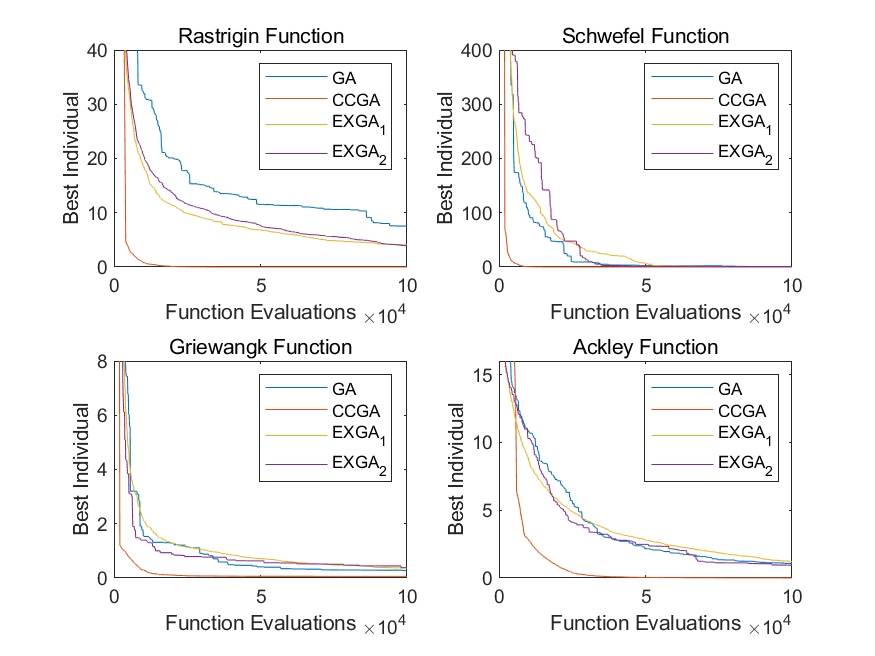
\includegraphics[width=0.9\textwidth]{img/extension_plot.png}
    \caption{The figure produced to demonstrate the extension produced for this assignment.}
    \label{fig:extension_plot}
  \end{figure}
